This section presents a simulation analysis of the various architectures based on the two data sets. 
We assess each variant in two different ways. First, for any method with an evaluative model we  measure the prediction accuracy of the EM. We compare the actual outcomes in a test set with the EM's prediction as to whether it is more likely to succeed or fail (output set at a threshold of 0.5). This gives us a confusion matrix from which we can calculated sensitivity, specificity and F1 score. Second, since a robot can only execute one grasp, we can measure the proportion of successful top-ranked grasps for any method. In each analysis the test set effectively replaces the Generative Model as it contains, for any scene, a complete list of grasps. Thus TS1 contains grasps proposed by GM1 and TS2 contains grasps proposed by GM2. This allows us to simulate the effect of different generative models on performance. 

We performed both analyses and the results are given in Table~\ref{table:Results-sim}. When assessing pure GM architectures, we can only measure the top ranked grasp success, since the GMs give a grasp likelihood according to the generative model not a probability of success. 

The main findings are as follows. First, of the pure generative models GM2 outperforms GM1, with top ranked grasp successes of 79.05\% and 69.53\% respectively. Second, the GEA architectures all outperform both pure GM architectures, starting at 87.85\% of grasps succeeding (V3 based on proposals from GM1 and evaluation by EM3 trained on TS1). Third, the increase in training set size (adding GM2 to GM1) yields a small improvement, with reductions in the residual grasp failures of 1.12\%-9.55\% when comparing the same architectures under different training conditions. All the above results for GEA architectures use GM1 as the generative model. We can measure the effect of substituting this by GM2. This yields a further 0.43\% to 1.82\% reduction in error over GM1 under the same training conditions (training with TS1 and TS2). 

It is informative to consider the relative size of the residual number of failed grasps relative to the baseline (pure generative model using GM1). We can see that overall the best model (V11) has just 31\%  of the failures that accrue to V1 (GM1).

%Recall that the generative-evaluative architecture (GEA) comprises both the generative model (GM) and the evaluative model (EM). 
%We can evaluate aspects of these separately. After training, the EM was used to predict grasp outcomes in the test set. This comprised 1,241 scenes with 76,213 grasps. Of these, 40,243 succeeded and 35,970 failed. Our analysis is given in Table~\ref{fig:predictions}. The sensitivity is 0.84 and the specificity 0.71. The F1-score is 0.802.
%\begin{table}[b]
%\centering
%\caption{Confusion matrix for prediction on simulated data.}
%\label{fig:predictions}
%\begin{tabular}{|c|c|c|c|c|c|}
%\hline
% & & \multicolumn{4}{c|}{Prediction} \\ \cline{3-6}
%      & & \multicolumn{2}{c|}{\#} & \multicolumn{2}{c|}{\%} \\ \cline{3-6}
%  &  & Succ         & Fail         & Succ         & Fail         \\ \hline
%\multirow{ 2}{*}{Ground Truth} \newline & Succ & 33890      & 6353       & 84\%     & 16\%       \\ \cline{2-6}
% &Fail & 10339      &  25631    & 29\%     &  71\%   \\ \hline
%\end{tabular}
%\end{table}
% In this context, precision is the fraction of correctly labeled grasps among those predicted to be of a certain class (success or failure). Recall stands for the fraction of relevant grasps that have been identified correctly among all grasps that belong to that class. The results show a high recall rate for successful grasps, and there are relatively more false positives than false negatives. This necessitates pairing our evaluative neural network with a generative model rather than a random grasp generator, which would likely result in very low quality grasps and consequently, more false positives. 

%To test our generative-evaluative learning architecture we compared the grasp it proposes to the grasp proposed by the generative learner alone. Since \citet{kopicki2015ijrr} showed a 77.7\% success rate with the original generative algorithm we generated a new test set that contained both more challenging objects and placed them in challenging poses. The difficulty single-view grasping with a depth camera depends greatly on the pose of the object relative to the camera. The set comprised 40 test objects (Figure~\ref{fig:real-objects}) and another six training objects. The training objects were used by the human to demonstrate ten example grasps (Figure~\ref{fig:generative-training}). The 40 test objects were used to generate 49 object-pose pairs. From the 40 objects, 35 belonged to object classes in the simulation dataset, while the remaining five do not. 

\begin{figure}[t]
  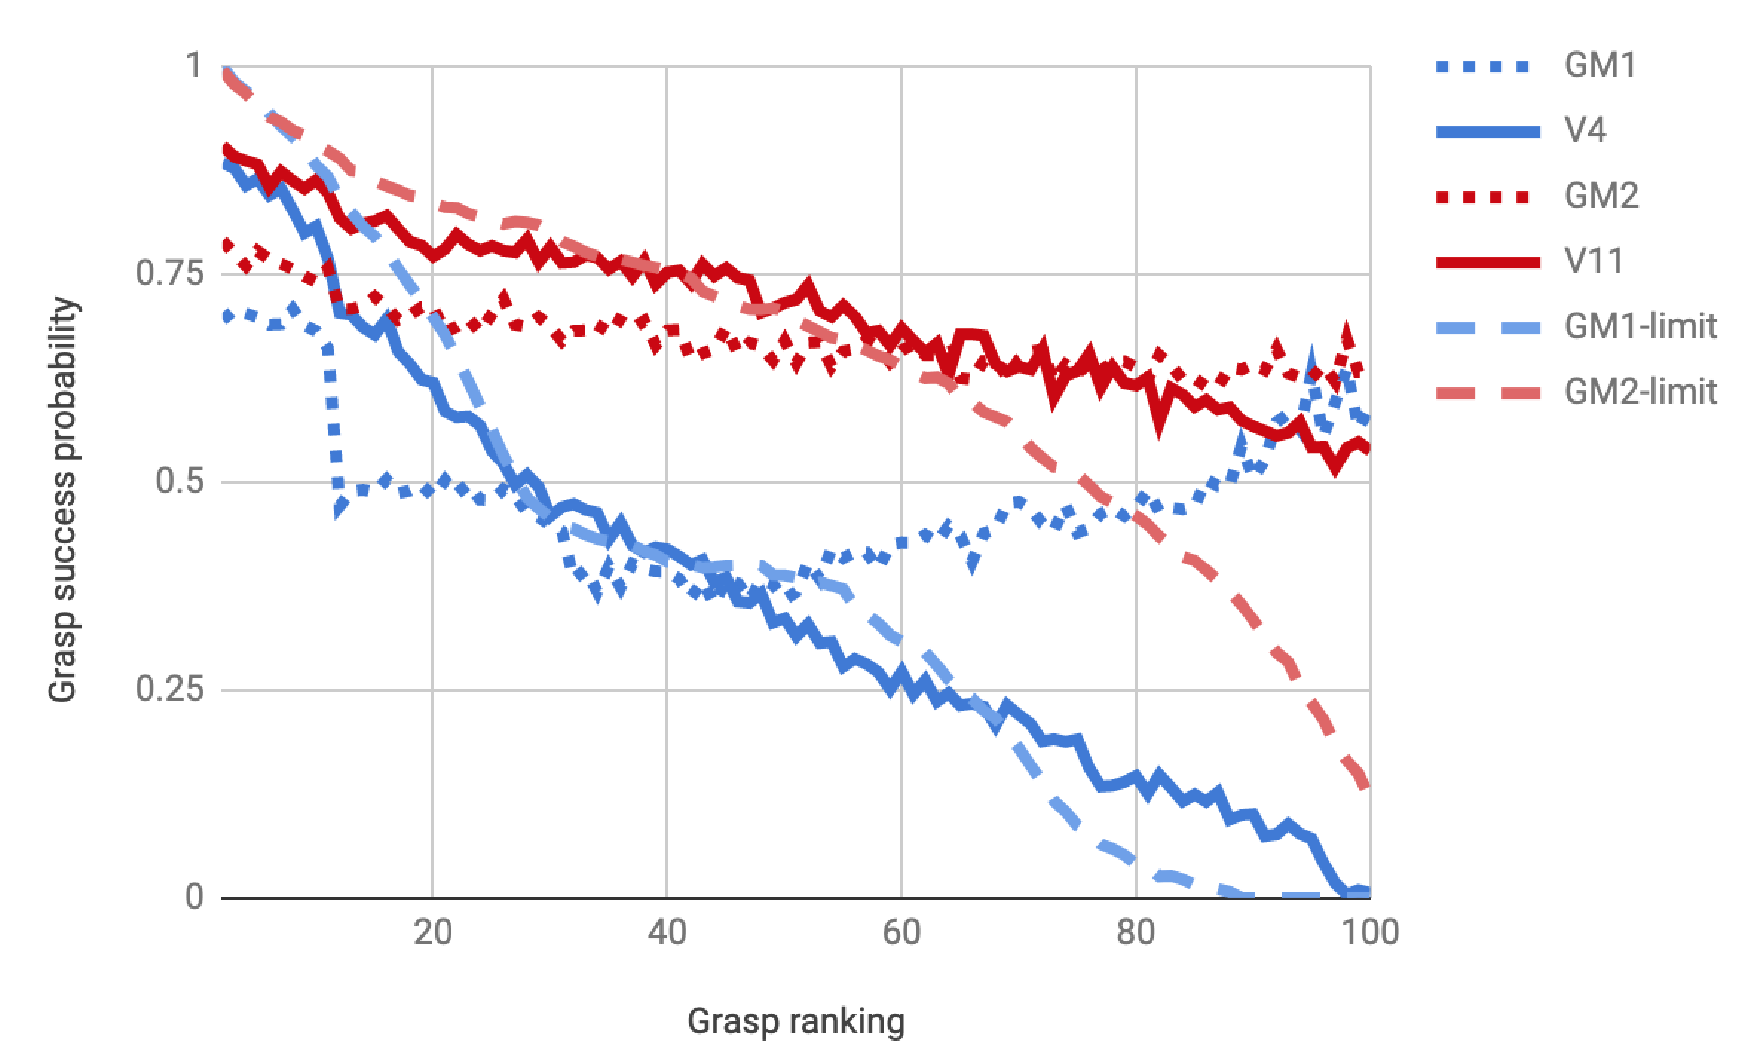
\includegraphics[width=\linewidth]{images/successvsranking.pdf}
  \caption{THIS FIGURE IS FOR OLD DATA. WE SHULD REDRAW. Grasp success probability (in simulation) vs. grasp ranking.}
  \label{fig:successvsranking}
\end{figure}

%We compared the EM and GM rankings (Figure~\ref{fig:successvsranking}). The x-axis shows the ranking. The y-axis shows the average actual success rate over all scenes (1,241 test, 7,311 training). When ranked by the EM, the grasp success probability falls nearly monotonically, as is desirable. On the other hand, the likelihood-based ranking of GM results in many good grasps being low-ranked. We also wish to know whether the grasps recommended by the EM and the GM have different grasp success rates. The success rates of the top-ranked grasps are 71.59\% (GM) and  84.2\% (EM).
So far we have considered only Generative-Evaluative architectures where the Evaluative Model merely ranks the grasp proposals. We also investigated using the EM to improve these grasps proposals. This essentially boils down to searching the grasp space driven by the EM as the objective function. This can be done either by gradient descent or using simulated annealing.Lu et al. \cite{lu2017planning} proposed gradient ascent on the input grasp parameters to the EM with respect to the predicted success probability. They initialised with a heuristic grasp. We initialise with the best grasp proposed by the GEA. 

We ran 20 and 100 epochs of gradient ascent on the EM network inputs. Although predicted success rate rises, the success rate in simulation declines. After 20 epochs it is 1.3\% lower and after 100 epochs it is 4.8\% lower than the actual success rate of the initial grasp. This suggests that optimising dexterous grasps by the EM is non-trivial, perhaps because of the high-dimensionality of the grasp space. We speculate that initialising with a random grasp would be even worse.

\begin{table*}[]
\centering
\begin{tabular}{|l|l|l|l|l|l|l|l|l|l|l|}
\hline
Variant \# & \multicolumn{2}{|c|}{Selected grasp} &  Succ \% & Residual Fails & Test set / GM& \multicolumn{5}{|c|}{Prediction Performance} \\ \hline
 & Succs & Fails &  & as \% of V1 fails &  & TP & FP & TN & FN & Accuracy \\ \hline
V1 & 1070   & 469 & 69.53\% & 100\% & GM1 & - & - & - & - & - \\ \hline
V2 &  781   & 207 & 79.05\% & 69\% & GM2 & - & - & - & - & - \\ \hline
V3 & 1352 & 187 & 87.85\% & 40\% & GM1 & 37840 &	12226 & 39211 & 10244 & 77.42\% \\ \hline
V4 &  1361 & 178 & 88.43\% & 38\% & GM1 & 40234 &	14475 & 36962 & 7850 & 77.57\% \\ \hline

V5 & 1361 & 178 & 88.43\% & 38\%& GM1 & 39603 & 14122 &37315 & 8481	& 77.29\% \\ \hline

V6 & 1375 & 164 & 89.34\% & 35\% & GM1 & 37584 &	11514 & 39923 &10500	& 77.88\% \\ \hline
V7 & 1363 & 176 & 88.56\% & 38\% & GM1 & 39332 &	12020 & 39417 & 8752 & 79.13\% \\ \hline
V8 & 1378 & 161 & 89.54\% & 34\% & GM1 & 37832 &	11361 & 40076	& 10252 & 78.28\% \\ \hline
V9 & 887 & 101 & 89.78\% & 34\% & GM2 & 61866 &	11454& 38847& 11970 & 81.13\% \\ \hline
V10 & 893 & 95 & 90.38\% & 32\% & GM2 & 64309 &	12517 & 37784 & 9527 & 82.24\% \\ \hline
V11 & 894 & 94 & 90.49\% & 31\% & GM2 & 61611 & 9792 & 40509 & 12225 & 82.26\% \\ \hline
V12 & & & & & & & & & & \\ \hline
V13 & & & & & & & & & & \\ \hline
V14 & & & & & & & & & & \\ \hline
V15 & & & & & & & & & & \\ \hline
V16 & & & & & & & & & & \\ \hline
V17 & & & & & & & & & & \\ \hline
\end{tabular}
\caption{Simulation results for all variants tested.}
\label{table:Results-sim}
\end{table*}


%A pure generative model architecture (GM) and the generative-evaluative architecture (GEA) were evaluated using a paired trials methodology. Each was presented with the same object-pose combinations. Each architecture generated a ranked list of grasps, and the highest ranked grasp was executed. The highest-ranked grasp based on the predicted success probability of the network is performed on each scene. A grasp was deemed successful if, when lifted for five seconds, the object then remained stable in the hand for a further five seconds before being automatically released. The success rate for GM was 57.1\% and for GEA it was 77.6\%. The successes and failures for each method were recorded and are summarised in Table~\ref{tab:robot-results}. A two-tailed McNemar test, for the difference between success rates for paired comparison data, was performed and the difference between the two algorithms has a $p$-value of 0.0442, and so is statistically significant. A selection of grasps where the two methods performed differently are shown in Figure~\ref{fig:successfail}.

% OLD TABLE
%\begin{table}
%\begin{center}
%\caption{Results of the real robot paired comparison trial.}
%\begin{tabular}{|c|c|c|c|}  \hline 
%          &                & \multicolumn{2}{ c |}{ GM} \\ \hline
%          &                & \# succs & \# fails  \\  \hline
 %GEA  & \# succs &  23 &  15  \\
 %         & \# fails    &  5   &   6   \\ \hline
%\end{tabular}
%\end{center}
%\label{tab:robot-results}
%\end{table}

%Training parameters for network. Training of example grasps for learning from demonstration. Creation of real test data set. Paired comparisons methodology with vanilla LFD algorithm (pose + object + camera view).
%
%The actual grasping tests have been performed on the real robot. 